
\chapter{Conclusion \& Future Work}
\label{ch:conclusions}

\section{Further Development of Monte Carlo Disorder Models for {\CZTS}}\label{eris_future_work}
So far from our simulations we are seeing clear clustering of Cu and Zn ions, such as that shown in figure \ref{eris_spatial_disorder}b. This is in agreement with a previous study performed for CZTS using a motif-based Hamiltonian and Monte Carlo simulations \cite{Lany_CZTS}. In this particular study the authors report on an entropically driven clustering of cations from their simulations. The radial distribution function (RDF) we showed in figure \ref{RDF_Z-Z} also indicates clustering of Zn ions with increased disorder due to the emergence of a new nearest neighbour peak in the Zn-Zn RDF when evolving the system from an initially perfectly ordered lattice.

Our study so far has focused on developing methods to gauge the point at which the system has reached its equilibrium amount of Cu-Zn disorder at the given simulation temperature, before we go on to extract thermodynamic information by averaging over data obtained from subsequent evolution of the system. The first method we attempted was to compare the RDF of a system evolved from an ordered initial lattice to that evolved from an initial disordered lattice. We would then use the principle that a system evolved from any initial configuration should eventually reach the same final configuration once the system has equilibrated to gauge when the system has equilibrated. The RDF can be used as a measure of long-range structural order so we could consider the point at which the two RDFs are the same (within a range of error) to be the point at which the system has attained its equilibrium configuration. However, so far from our simulations it seems that the system takes a considerably longer time (in terms of Monte Carlo simulation steps) to evolve from an initial disordered lattice. This can be seen in the RDFs shown in figure \ref{RDF_Z-Z_equil_check}, where the RDF of the system evolved from a disordered lattice changes very little from the RDF of the initial configuration compared to that evolved from an ordered lattice. 

We next tried tracking the variance in the distribution of the electrostatic potential of Sn ions for the system evolved from an ordered lattice. For a perfectly ordered lattice, the variance is zero due to there being only one unique chemical environment for Sn in perfectly ordered CZTS. From these simulations, where some of the results were shown in figures \ref{variance_with_MCS} and \ref{variance_with_MCS_1000}, it appears that the system evolved from an ordered initial lattice reaches an equilibrated configuration after a fairly modest number of Monte Carlo steps of approximately 2000 steps in total. This suggests that when starting from this particular configuration, around 2000 steps could be a sensible number of steps to run for the simulation for before collecting data on thermodynamic information about the system.

Our study so far has also focused on developing methods to quantify the Cu-Zn disorder present in large and three-dimensional systems. We have initially just used the RDF for Cu-Cu pairs and Zn-Zn pairs, as discussed above, but we intend to develop more methods. This initial method is based on using the characteristic clustering of Cu and Zn ions as a measure of disorder. This principle could also allow us to use the clusters themselves as a measure of disorder, and possibly another way to gauge if our system has attained its equilibrium configuration. For this development, we will attempt to measure the size of Zn clusters present in the system and then count the number of clusters of each size. The point at which the number of each cluster size does not change after a large number of simulation steps could be considered the point at which the system has reached an equilibrated extent of Cu-Zn disorder.

In addition, there are other methods that have been used in the literature to quantify Cu-Zn disorder in CZTS, which we could try to apply to our simulations. One method that has been used to quantify short-ranged cation disorder in CZTS involves studying how the local environments of S anions deviate to that in the perfectly ordered crystal lattice \cite{Lany_CZTS}. In the case of the ordered crystal, one S anion should be surrounded by two Cu ions, one Zn and one Sn. However as Cu and Zn ions substitute with thermodynamic disorder, a number of different motifs are possible. For example, one S ion could instead be surrounded by one Cu and two Zn ions or three Cu ions and no Zn ions in the first coordination sphere. In reference \citenum{Lany_CZTS}, cation disorder is quantified by counting the number of each type of motif present.
This treatment will only capture very short-ranged disorder so we may wish to build upon the methodology of the authors in reference \citenum{Lany_CZTS} to look at the deviation in the local environment of S anions to next nearest neighbour and next-next-nearest neighbour cations. Or, as we fix Sn ions in our simulations and do not initially include S ions in our Monte Carlo simulations, the local environment of Sn ions could be a more sensible way for us to perform the same type of analysis.

However, the most common method in the literature to quantify Cu-Zn disorder experimentally is to measure the site occupancy of sites which, in a more ordered system, should be preferentially occupied specifically by Cu or Zn. A recent example of such a study where the temperature dependence of Cu/ Zn ordering in CZTSe is measured and quantified in such a way using anomalous diffraction is given in reference \citenum{Schorr_new}. In this study the authors define an order parameter Q, shown in equation \ref{order_param}, where for example Cu$_{2c}$ indicates the number of 2c sites that are occupied by Cu ions, which corresponds to the correct position for an ordered CZTS lattice. Likewise, Zn$_{2d}$ corresponds to the same situation for sites that should be occupied by Zn in the perfectly ordered system.
\begin{equation} \label{order_param}
Q = \frac{[Cu_{2c} + Zn_{2d}] - [Zn_{2c} + Cu_{2d}]}{[Cu_{2c} + Zn_{2d}] + [Zn_{2c} + Cu_{2d}]}
\end{equation}
In a completely disordered system, 2c and 2d sites are occupied by an equal number of Cu and Zn ions, but as a system becomes more ordered Cu and Zn ions preferably occupy the correct site. For a perfectly ordered system, Q=1 and for a completely disordered system Q=0. In our simulations, we could attempt to implement something similar by studying the occupancy of the crystallographic sites by considering the original perfectly ordered unit cells the supercell lattices in our simulations were constructed from.

Once we have fully established our methods for gauging when our system has equilibrated and for quantifying structural disorder, the next important step is to investigate the size dependence of our simulation-derived properties. This will be done by using our methods for quantifying disorder. We will vary the system size and study how this effects our order parameters, with the aim of determining a minimum system size for the equilibrium amount of disorder at each temperature to no longer vary with increased system size. Once a suitable system size has been determined, we will then go on to extract information on band tailing in CZTS due to Cu-Zn disorder. We intend to do this by studying the distribution of the electrostatic potential of Sn ions in the various disordered systems. We will investigate how the density of states (DOS) of Sn ions in a disordered system shifts relative to that of a perfectly ordered system. As the electronic environment is related to the ionic environment we will infer that the electronic DOS will be shifted in the same way as the ionic DOS. From this we aim to extract the amount one would expect the electronic DOS to tail into the band gap of the perfectly ordered system, such as that shown in figure \ref{pankove_elec_fluc}.


\section{Predicting the Photovoltaic Performance of Other Metal Sulfide Materials}\label{sulfosalts_proj}
As discussed in section \ref{sulfosalts_intro}, another component of this study is to predict the optoelectronic properties of other materials, which have currently received little or no attention for PV, to determine the likely performance of the materials for this application. The three candidate materials were: enargite ({\enargite}), stephanite ({\stephanite}) and bournonite ({\bournonite}). These materials are all classed as sulfosalt minerals and an overview of their known properties was given in section \ref{sulfosalts_intro}. The candidate PV materials were originally selected based on the possibility of ferroelectricity due to their polar space group and associated ferroelectric-photovoltaic phenomena, which could open up new possible pathways for high performance PV devices. However, currently in the study it is only the optoelectronic properties relevant for PV applications that are being studied.

\begin{figure}[h!]
  \centering
    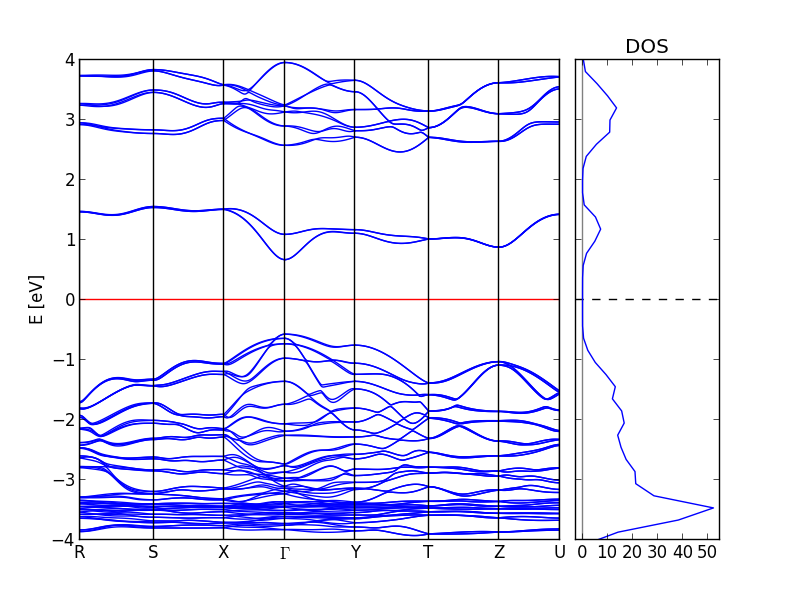
\includegraphics[width=0.9\textwidth]{figures/enargite_band_structure.png}
    \caption{Band structure and density of states (DOS) of enargite ({\enargite}) calculated using the HSE06 functional with spin-orbit coupling. The atomic structure is obtained from experimental lattice parameters with internal atomic positions optimized with the HSE06 functional.}
  \label{enargite_band_structure}
\end{figure}

\begin{figure}[h!]
  \centering
    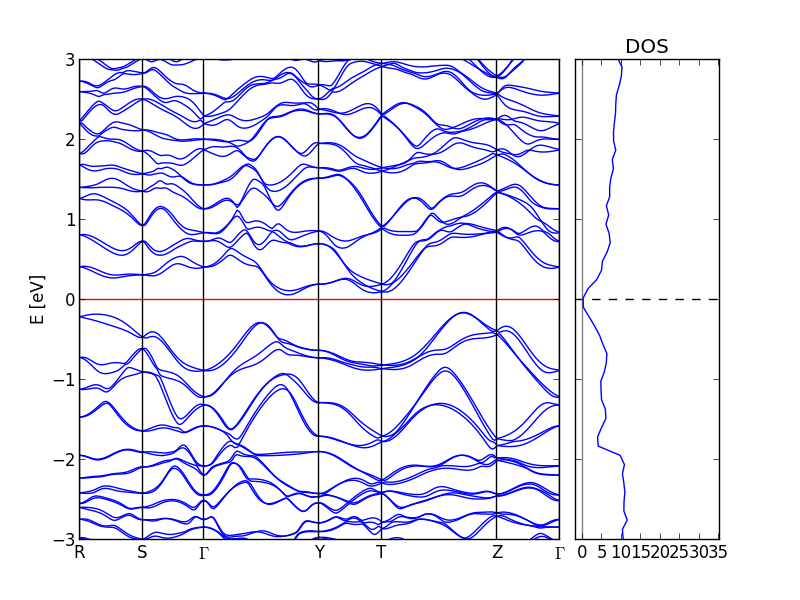
\includegraphics[width=0.9\textwidth]{figures/stephanite_band_structure.png}
    \caption{Band structure and density of states (DOS) of enargite ({\stephanite}) calculated using the HSE06 functional with spin-orbit coupling. The atomic structure is obtained from experimental lattice parameters with internal atomic positions optimized with the HSE06 functional.}
  \label{stephanite_band_structure}
\end{figure}

One of the first key material properties for PV applications mentioned in section \ref{PV_properties} was the band gap of the material; both its magnitude relative to the solar spectrum and whether it is direct or indirect in nature. Therefore we firstly calculate the band structures of the materials and these are shown in figures \ref{enargite_band_structure}, \ref{stephanite_band_structure} and \ref{bournonite_band_structure} for enargite, stephanite and bournonite respectively.
Electronic structure calculations in this study are performed using the HSE06 functional \cite{HSE} as implemented in the FHI-aims software package \cite{aims, aims_hybrids, aims_parallel}, with the inclusion of spin-orbit interaction 
%\cite{aims_SOC}
.
Initial geometries are taken from high-quality X-ray diffraction data from the Inorganic Crystal Structure Database (ICSD)\cite{icsd} for enargite and bournonite and the resolved crystal structure from single crystal X-Ray diffraction measurements performed by Professor Mark Weller at the University of Bath on a natural sample of stephanite during a previous study. Geometry optimization of the structures are then performed allowing only the ionic positions to relax, holding the unit cell parameters constant.
An evenly spaced 4x4x4 \textit{k}-points grid centred on the $\Gamma$-point is used for the \textit{k}-space sampling of the first Brillouin zone as this was found to be sufficient for the total energies of the systems to converge to within 1 meV in our previous study. Convergence plots from this study are shown in Appendix \ref{k-points}.
Default `tight' accuracy convergence settings of the FHI-aims code were used for the basis sets and geometry relaxations were performed to obtain optimized structures using the Broyden-Fletcher-Goldfarb-Shanno (BFGS) optimization algorithm as implemented in the FHI-aims code \cite{aims} until forces on the atoms converged to within a tolerance of $10^{-3}$ eV/ $\AA$. Band structures were then plotted along the paths of high symmetry for each type of crystal structure, shown in Appendix \ref{paths}. For band structure calculations the density of the \textit{k}-points grid was increased to 8x8x8.

\begin{figure}[h!]
  \centering
    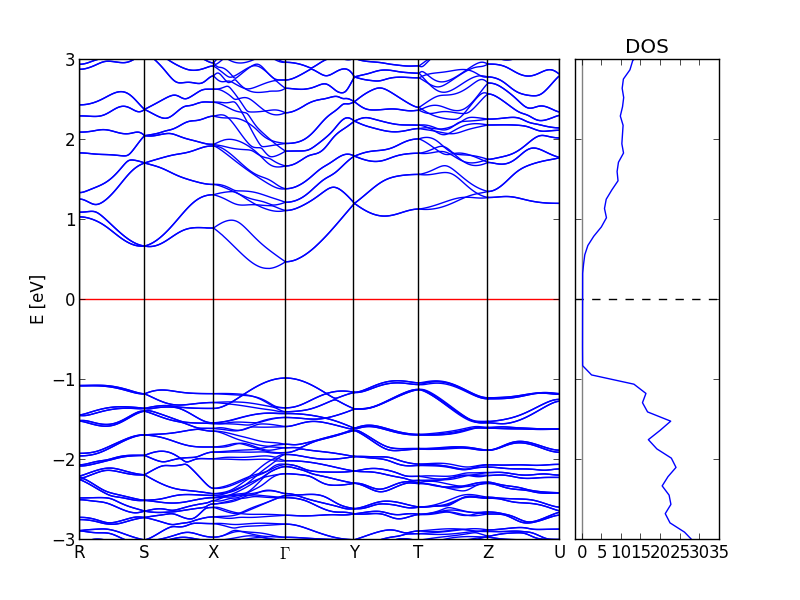
\includegraphics[width=0.9\textwidth]{figures/bournonite_band_structure.png}
    \caption{Band structure and density of states (DOS) of bournonite ({\bournonite}) calculated using the HSE06 functional with spin-orbit coupling. The atomic structure is obtained from experimental lattice parameters with internal atomic positions optimized with the HSE06 functional.}
  \label{bournonite_band_structure}
\end{figure}

\begin{figure}[h!]
  \centering
    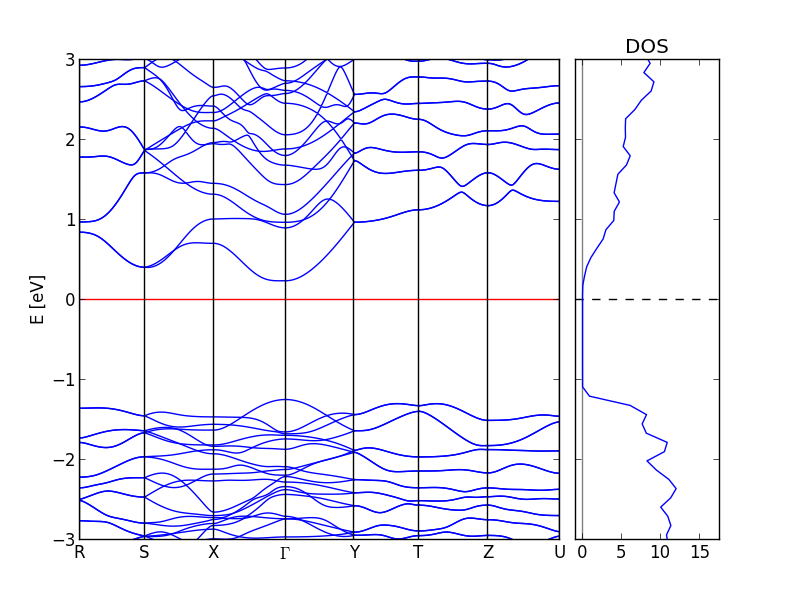
\includegraphics[width=0.9\textwidth]{figures/bournonite_band_structure_no_SOC.png}
    \caption{Band structure and density of states (DOS) of bournonite ({\bournonite}) calculated using the HSE06 functional without spin-orbit coupling. The atomic structure is obtained from experimental lattice parameters with internal atomic positions optimized with the HSE06 functional.}
  \label{bournonite_band_structure_no_SOC}
\end{figure}

From our calculations, enargite has a direct band gap of 1.24 eV. This is within the range of experimental values obtained for the band gap in the literature and is also in good agreement with UV-vis measurements on a natural sample of enargite that we performed during a previous study, which gave a value of approximately 1.2 eV for the band gap. Although it should be noted that this natural sample was found to contain Sb impurities. The value we calculate is also not too far from the 1.32 eV calculated in a previous theoretical study using G$_0$W$_0$@HSE06 \cite{Zunger}.
For stephanite we calculate an indirect band gap of 0.22 eV. As far as we are aware there are no other theoretical predictions for the band gap of this material but our value is considerably less than experimental values obtained in the literature \cite{Dittrich1}  and our UV-vis measurement performed in a previous study which all give a value of around 1.6 eV.
For bournonite, we calculate an indirect band gap of 1.37 eV, which is in quite good agreement with experimental values in the literature of 1.23 \cite{Dittrich1} and 1.31 \cite{bournonite} eV. However to our knowledge there are currently only calculated values for the band gap of bournonite in the literature using GGA and GGA+U methodologies. From the calculated band structure for bournonite shown in figure \ref{bournonite_band_structure}, it appears that the material could exhibit conduction band spin splitting as a consequence of spin-orbit coupling. This is often referred to as Rashba splitting. The long carrier lifetime and diffusion length observed in organometal halide perovskite solar cells has been postulated to be linked to Rashba splitting in the band structure of these materials \cite{Rashba_MAPI, Rashba_MAPI_aron}. In these works the authors suggest that the rate of electron-hole recombination could be reduced due to the spin-forbidden transition, thereby resulting in enhanced carrier lifetimes. 
Therefore, although the band gap we predict for bournonite is slightly indirect, it could be possible that this property could be beneficial for PV applications. The next step in investigating the optoelectronic properties of bournonite is to determine if the observed band splitting is in fact Rashba splitting. So firstly the band structure has been re-calculated with spin-orbit interaction omitted to see if the splitting is caused by spin-orbit coupling and from figure \ref{bournonite_band_structure_no_SOC} it does appear that the splitting of the conduction band has disappeared.

However, it has been suggested that the Shockley-Queisser (SQ) theoretical efficiency limit of a solar cell based on the value of direct band gap is not a sufficient screening criteria for candidate PV materials \cite{SLME}. The authors instead suggest an alternative metric called the `spectroscopic limited maximum efficiency' (SLME), which takes into account the band gap, the shape of the optical absorption spectra and the material-dependent non-radiative recombination losses. In the same work the author's show that from their metric many materials have a maximum efficiency limit less than that predicted by SQ, this is illustrated in figure \ref{SLME}. Interestingly, the authors also find that some materials with similar band gaps (and therefore would have similar SQ limits) have very different theoretical limits from their metric. Therefore a more thorough evaluation of the potential of the candidate materials for applications in PV could be achieved by extending our investigation to encompass the SLME metric.

\begin{figure}[h!]
  \centering
    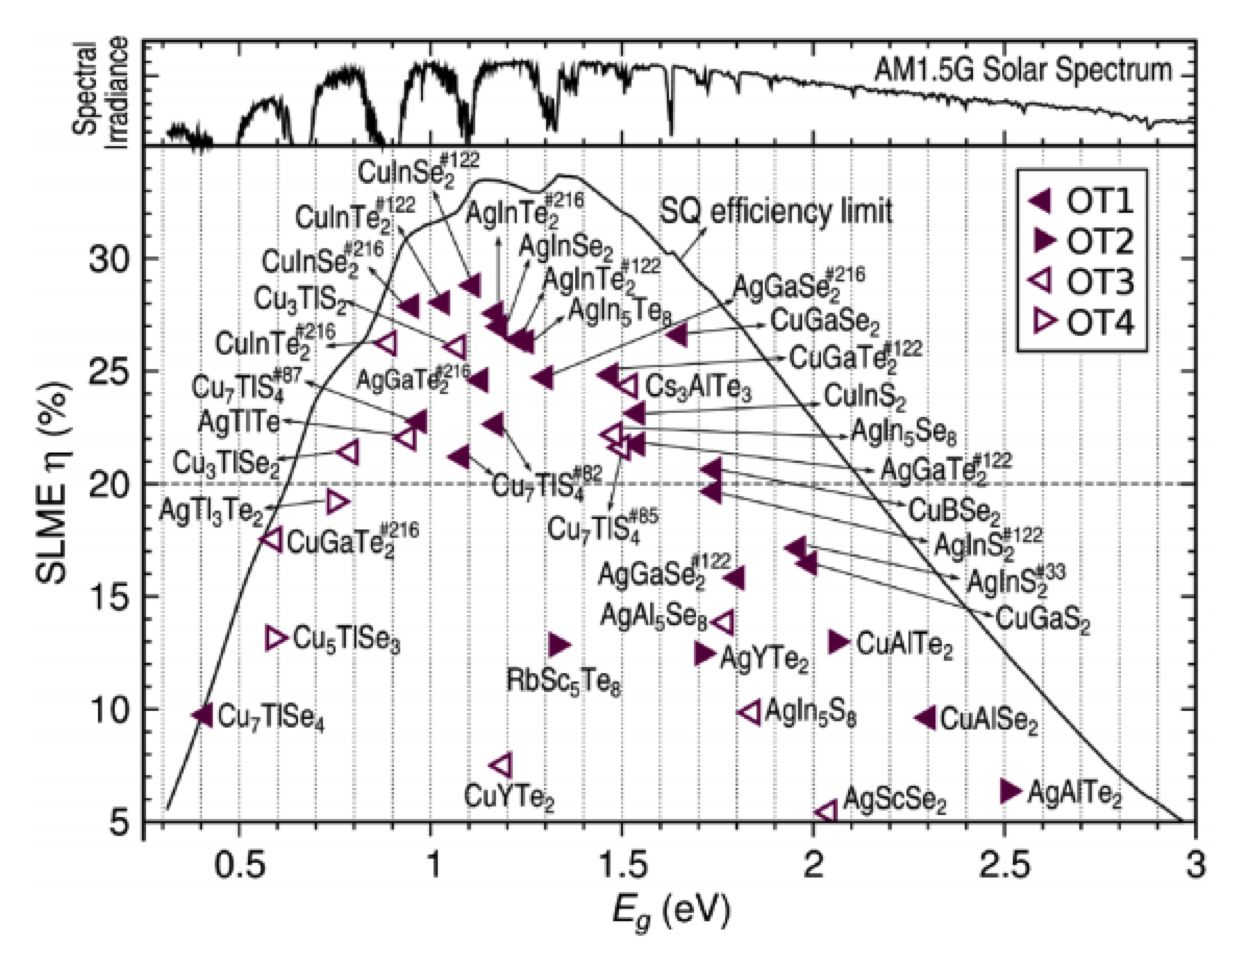
\includegraphics[width=0.8\textwidth]{figures/SLME.png}
    \caption{Spectroscopic limited maximum efficiency (SLME), $\eta$, versus the minimum band gap, E$_g$, for I-II-VI chalcopyrite materials of thickness L= 0.5 $\mu$m (triangles). The Shockley-Queisser (SQ) efficiency limit is shown by the line. Figure taken from reference \citenum{SLME}.}
  \label{SLME}
\end{figure}



%\section{Formation Energy of Sulfur Vacancies in Metal Sulfides}\label{Vs_proj}
%As discussed in section \ref{defects_in_PV}, defects in a solar absorber material can heavily impact on the performance of a photovoltaic device composed of that material. We performed calculations of the formation energy of the charge neutral Cu-on-Zn and Zn-on-Cu anti-site defect pair, [$Cu_{Zn}^- + Zn_{Cu}^+$], in order to parameterize our Monte Carlo simulations of thermodynamic Cu-Zn disorder, which was discussed in section \ref{MC_DFT}. However, as mentioned in section \ref{bottlenecks}, sulfur vacancies in {\CZTS} have been predicted to give defect states deep within the band gap and so their presence would be very detrimental to device performance. Although the formation energy for this particular defect has been predicted to be fairly large compared to for example $Cu_{Zn}^-$ or $Zn_{Cu}^+$ antisites, it is possible that previous studies may have underestimated the likelihood of the formation of sulfur vacancies in {\CZTS} due to the volatility of sulfur and the typical annealing conditions of CZTS. We have therefore begun calculations of the formation energy of a sulfur vacancy in {\CZTS }. This defect can take on three different charge states: $V_{S}^{0}$, $V_{S}^{+1}$ and $V_{S}^{+2}$, where electron occupancy varies from two to one to none respectively. 
%\begin{figure}[h!]
 % \centering
  %  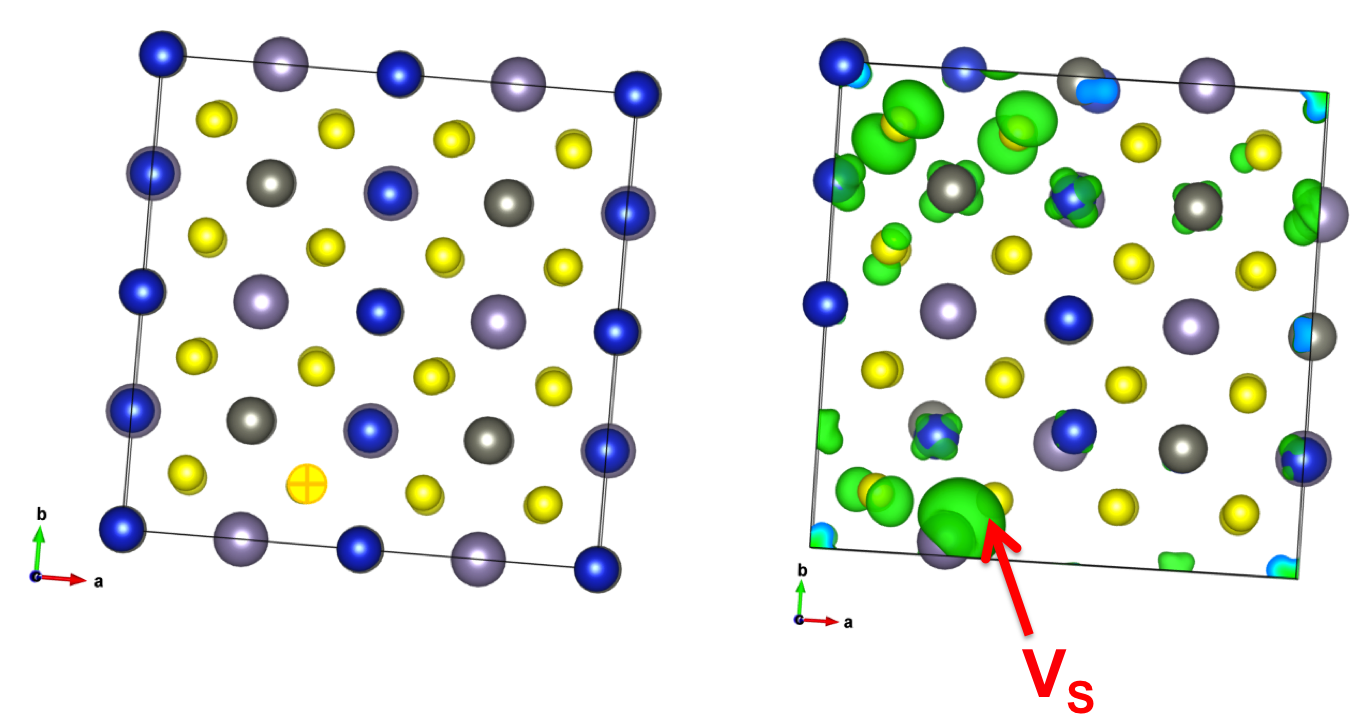
\includegraphics[width=0.9\textwidth]{figures/V_S-neutral-PARCHG.png}
  %  \caption{Perfect {\CZTS } supercell with S anion removed to form a sulfur vacancy (V$_S$) indicated by a crosshair (left) and the calculated partial charge density of two excess electrons present for the charge neutral V$_S$ (right).}
 % \label{V_S-neutral-PARCHG}
%\end{figure}
%\begin{figure}[h!]
%  \centering
%    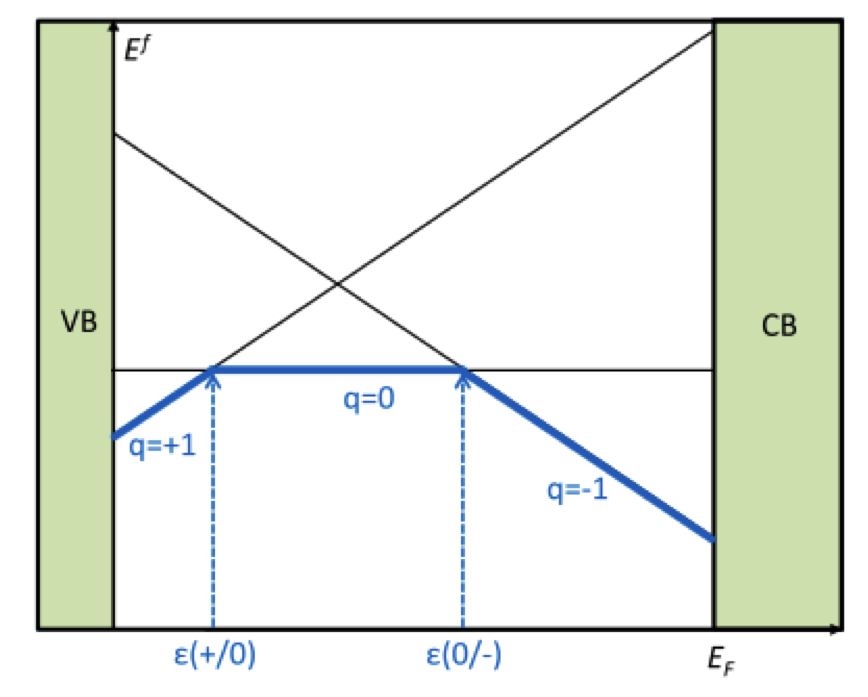
\includegraphics[width=0.6\textwidth]{figures/defect_calc_example.png}
 %   \caption{Schematic illustration of defect formation energy ($E_f$) versus Fermi level ($E_F$) for an amphoteric defect that can occur is three charge states q: +1, 0 and -1. The thick blue line indicates the most energetically favourable charge state for a given fermi level. Figure taken from reference \citenum{defects_encyclopedia}.}
%  \label{defect_calc_example}
%\end{figure}
%The methodology and need to go beyond standard density functional theory (DFT) to hybrid DFT in order to perform calculations to predict the defect properties of semiconductors was discussed in relation to the calculation of the [$Cu_{Zn}^- + Zn_{Cu}^+$] in {\CZTS} to parameterise our Monte Carlo simulations in Appendix \ref{Cu-Zn_defects_calc}. However, for the present discussion it is worth restating the general formula for defect formation energy again where $\Delta H_{D,q}$ is the total energy of the supercell containing the defect in charge state q, $E_H$ is the total energy of an equivalent supercell of the perfect host crystal without the defect. The chemical potential $\mu_{\alpha}$ describes the energy of the atomic reservoir of the atoms $\alpha$ removed from or added to the host crystal when the defect forms. For charged defects, where q $\neq$ 0, $E_F$ describes the energy of the reservoir of electrons, which is usually considered to be somewhere between the valence band maximum and conduction band minimum, but can be tuned by an applied bias. Unlike in the case of the charge neutral antisite pair, when calculating the formation energy of a sulfur vacancy the defect is not charge neutral. The full formula applies in this case and charge corrections must be applied to correct for Coulombic interactions between periodic images of the defect when using the supercell method in periodic DFT \cite{defects_Lany}.
%\begin{equation} \label{defect_formation}
%\Delta H_{D,q}(E_F, \mu) = [E_{D,q} - E_H] + \sum_\alpha n_{\alpha}\mu_{\alpha} + q \cdot E_F
%\end{equation}
%We have currently obtained total energies for the three possible charge states of the sulfur vacancy is CZTS and the charge density of the charge neutral defect is shown in figure \ref{V_S-neutral-PARCHG}. Next we need to apply charge corrections to the total energy of the two supercells containing the charged defects. We will then go on to calculate the formation energy using a value for the sulfur chemical potential that is representative of typical annealing condition, using the model developed in reference \citenum{Adam_sulfur}. 
%Formation energy for sulfur vacancies in the various charge states will then be calculated as a function of Fermi level to determine which charge state has the minimum formation energy across the range. A schematic of such a plot is shown in figure \ref{defect_calc_example}, although this particular example is for a defect than can take on charge states of q: +1, 0 or -1 as opposed 0, +1 or +2 for a sulfur vacancy. If we find that sulfur vacancies are in fact likely defects in CZTS, may later go on to repeat the process for the sulfosalt materials discussed in section \ref{sulfosalts_proj} to determine if the defect is less likely to form or result in a less detrimental defect state in these materials.



%\section{Intrinsic Band Gap Broadening in {\CZTS}}\label{Eg_broadening_proj}
%In section \ref{PV_properties}, both effective mass and dielectric function were discussed for the insight these properties can provide for the likely PV performance of a material due to the impact these properties can have on the mobility of charge carriers in that material. However these are certainly not the only features of a real material at finite temperatures that need to be considered to understand carrier mobility in a material. 
%Even in a perfect crystal, atoms are involved in some sort of thermal motion about their idealized equilibrium positions. The simplest model to describe this motion is the Einstein model where each atom vibrates independently and as a simple harmonic oscillator in the potential well created by the force fields of its neighbouring atoms. The field can never be precisely a quadratic well with spherical symmetry, but on average the approximation is reasonable, especially when only a very crude picture of thermal vibrations is sufficient or at fairly high temperatures, when the assumption that atoms vibrate independently of each other is more justified \cite{Ziman_solids}. In this model, the oscillations of the atoms can be expressed in terms of normal modes as they are independent of each other. Energies of these normal modes are then quantised, where a quantum of lattice vibration is referred to as a phonon \cite{fund_semi}.

%For a given crystal structure, there are 3N phonon modes, three of which are lower-energy acoustic branches and the rest are optical curves and where N is the number of atoms in the primitive unit cell. In the case of {\CZTS}, there are therefore 24 phonon modes. Calculated phonon dispersion curves for kesterite-structured {\CZTS} are shown in figure \ref{CZTS_phonons}.
%Along directions of high symmetry these phonons can be classified as transverse or longitudinal depending on whether their displacements are perpendicular or parallel to the direction of the wavevector respectively. In a solid the long wavelength transverse acoustic (TA) phonons are shear sound waves, while the longitudinal acoustic (LA) phonons are compressional sound waves. The velocities of these sound waves are determined by shear and bulk elastic moduli respectively. As it is usually easier to shear than to compress a crystal, TA phonons typically travel with lower velocities than LA phonons.  
%The atomic displacements from long wavelength acoustic phonons can correspond to a deformation of the crystal, this is referred to as deformation potential theorem. Such deformations will change the electronic energies at different points in the Brillouin zone. LA phonons always produce a change in the volume of the crystal, which affects all energy bands \cite{fund_semi}.

%\begin{figure}[h!]
 % \centering
 %   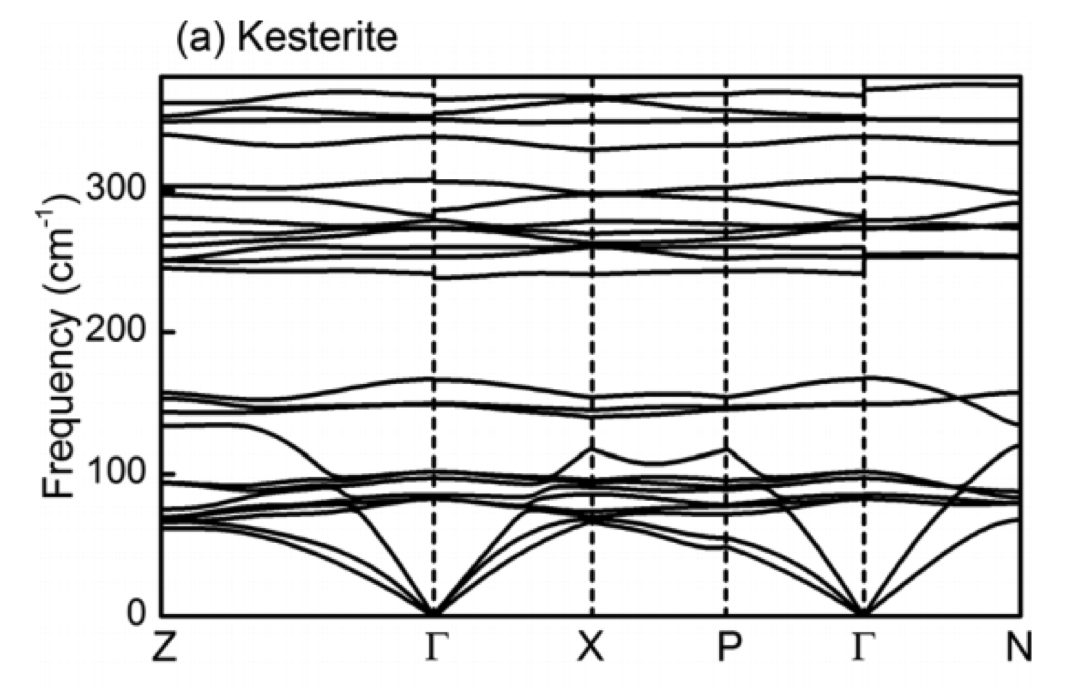
\includegraphics[width=0.7\textwidth]{figures/CZTS_phonons.png}
 %   \caption{Phonon dispersion curves of {\CZTS}.  Figure taken from \citenum{CZTS_phonons}.}
%  \label{CZTS_phonons}
%\end{figure}

%The interaction of charge carriers with phonons, often referred to as electron-phonon coupling, sets a fundamental limit on the mobility of charge carriers in a material in the absence of extrinsic scattering due to defects, impurities or interfaces \cite{fund_semi, MAPI_Eg_broadening}. 
%Thermal vibrations of the lattice atoms gives rise to a perturbation of the band edge \cite{thin_film_Boer}, although the interaction of charge carriers with phonons is currently still a subject of much debate \cite{MAPI_Eg_broadening16, MAPI_Eg_broadening17, MAPI_Eg_broadening}.
%Of all the various possible contributions to intrinsic band gap broadening from electron-phonon coupling, there is currently no clear picture of which mechanisms are active or the most dominant in determining the carrier mobility in a material \cite{MAPI_Eg_broadening}, however it could be argued that lowest energy phonon modes are likely to make the biggest contribution. A number of studies on non-polar inorganic semiconductors have examined the temperature dependence of the charge-carrier mobility \cite{MAPI_Eg_broadening21, MAPI_Eg_broadening22, MAPI_Eg_broadening23, MAPI_Eg_broadening24}, where the carrier mobility, $\mu$, was found to scale with $T^m$ where m has a value between -1.4 and -1.6. From theory, it is known that deformation potential scattering with acoustic phonons results in $\mu \propto T^{-\frac{3}{2}}$. Therefore several works in the literature suggest that electron-phonon coupling at room temperature is dominated by acoustic phonons \cite{MAPI_Eg_broadening16, MAPI_Eg_broadening17, MAPI_Eg_broadening24}. Looking again at figure \ref{CZTS_phonons}, the acoustic modes are the three that tend to zero at the gamma point.

%In on-going work, we aim to determine if the effect of the thermal motion of ions in perfect CZTS crystals could fundamentally limit carrier mobility and device performance. To do this, we have first computed the effect of volume on the band gap (the deformation potential) and have also calculated the elastic constant of bulk CZTS. So far, for CZTS we find that the band gap decreases as a result of lattice dilation, which is a trend observed in most typical semiconductors such as Si, Ge and GaAs \cite{MAPI_Eg_broadening}. This effect can be understood as a weakening of the bonds as ions are pulled apart and decreasing the separation of filled and empty states. For the next stage of this investigation, the elastic constant will be used to determine the magnitude of volume changes expected from thermal motion as a function of temperature. The deformation potential will then be used to determine the extent of band gap broadening expected to be caused by such changes in volume with temperature.
